\documentclass[10 pt]{article}

\usepackage{fontspec}
\defaultfontfeatures{Mapping=tex-text}
\setmainfont{Minion Pro}

%\usepackage{graphicx}
%\usepackage{fullpage}

\usepackage{lastpage, fancyhdr}
\pagestyle{fancy}
\lhead{Scott O'Connor}
\chead{Phil 234} 
\rhead{\emph{Meno}}
\lfoot{}
\cfoot{\thepage\space of \pageref{LastPage}} 
\rfoot{}

\thispagestyle{empty}


\begin{document}
\author{Phil 234}
\title{\emph{Meno}}
\maketitle

\section*{Overview}
The dialog begins with Meno, a Thessalian, asking whether virtue is teachable (70a1-4). Meno is ambitious. He wants to become a tyrant, i.e., run things. Someone else around. That is why virtue means a lot to him. Virtue was seen roughly as the set of qualities whose possession is required to a) govern a city well, and b) govern yourself well, c) govern a household well.  Meno is asking how this skill can be acquired. He offers three options. 1) You are born with it. 2) You acquire it through practicing it. 3) You acquire it by being taught it.

 There are folks like Gorgias who think that they can teach you how to be virtuous. Athenian political society was premised on the idea that it was teachable. You would apprentice with folk. You would pratice. If it cannot be taught, then  this has serious reprecussions for moral education . 

Larger epistemological concerns. It asks whether we can search for Socratic definitions. 


\section*{Socrates' Challenge}

Socrates claims that he does not know whether virtue can be taught because he does not know what it is (71b1--8). In making this claim, Socrates tells us that we must have an answer to the question `what is virtue?' before we can determine whether virtue is teachable. Recall that an answer to such a question is called a Socratic Definition. Socrates, therefore, is here articulating what is called the \emph{priority of definition}:
\begin{itemize}
\item In order to know what qualities x possesses, you must know what x is, i.e., the definition of x. 
\end{itemize}
He offers the following example: in order for you to know whether Meno is good-looking, rich, or well-born, you must know who Meno is. That is, if you do not know at all who Meno is, then you cannot know what qualities belong to Meno. This seems implausible. Suppose you are in a room with a red-haired stranger. Can't I know that the person has red hair without knowing who they are? Socrates will respond by asking what we mean by saying we can know that the person has red hair. Assume that the person's name is John. If you do now know who John is, then Socrates will claim that you cannot know that John has red hair just by looking at him. You can know, perhaps, that there is a person in a room with red hair. But that is quite different from knowing that \emph{John has red hair}. Since you don't know the person is John, you just couldn't know that John has red hair. 

Socrates assumes the following:
\begin{enumerate}
\item There is a distinction between essential and non-essential features, e.g., humans are essentially rational, but they are not essentially capable of laughter.
\item Essential features are explanatory of (some) non-essential features/
\end{enumerate}
So Socrates is assuming that being teachable is not the essence of virtue. If he did know the essence of virtue, he would know what follows on from that essence, including whether it is teachable. 

The dialog proceeds by discussing  various candidate definitions of virtue. During this initial discussion, Socrates strains to illustrate the requirements for a Socratic definition. He does so in two ways. He first has Meno try define virtue and illustrates the requirements by failure. He then gives a few successful definitions of color. This tells Meno how he should define virtue. Recall then the features of definitions: 
\begin{enumerate}
\item General
\item Univocal
\item Explanatory 
\end{enumerate}

\section*{The paradox of inquiry}
Socrates believes we must know what virtue is before knowing whether it is teachable. Meno challenges Socrates claim that we can inquire into the nature of anything. (80d5-80e5)


\begin{enumerate}
\item[P1] If you know x already, you cannot inquire into x. 
\begin{enumerate}
\item[] Read `inquire into x' as `inquire into the essence of x'. 
\item[] When people begin searching for something, they do not yet possess what they are searching. So if you know that you possess something, it makes no sense to say that you can search for it.
\end{enumerate}
\item[P2] If you do not know x, you cannot inquire into x (since X doesn't know what to search for).
\begin{enumerate}
\item If you do not know \emph{at all} what x is, then you cannot start to inquire into x...you will not not know how to start even looking.
\item If you do not know what x is, and if you stumble upon x, you will not know that what you stumbled upon is x, e.g., if you do not know who Meno is, but stumble upon him, then you will now know that the person you stumbled upon is Meno. 
\end{enumerate}
\item[P3] Either you know x or you do not. (Implicit Premise) 
\item[C] Therefore you cannot inquire into x.
\end{enumerate}

We have reached an impasse.  Socrates claims that we cannot find out whether virtue is teachable until we know what virtue is, i.e. know the essence of virtue.  But Meno argues that we cannot inquire into the essence of virtue if we know nothing at all about it. This is a serious impasses. It seems we must know at least something about virtue before we can investigate its nature. But it also seems that we cannot know anything about virtue without already knowing its nature. So, it follows that it is impossible to find out whether virtue is teachable. 

\section*{Socrates' response: The Theory of Recollection (TR)}
To solve the dilemma, Socrates must feasibly reject one of the premises. He does so by offering a theory of learning: what we call learning is recollecting things we already know ((81b3--c9).

The Slave Boy Example is meant to support the Theory of Recollection. The Slave Boy must find out how long the sides are of a 8 sq ft square. By being questioned by Socrates, the Slave Boy \emph{recollects} the correct answer (85d2-10) .

\begin{enumerate}
\item[A] S recovers the knowledge from within himself.
\item[B] Recovering knowledge for oneself that is in oneself is recollection. (Assumed)
\item[C] If S recollects what he knew, he either acquired that knowledge in the past or else always possessed it. 
\end{enumerate} 

Socrates' cross-examination of the slave boy is meant to prove A. This assumes:
\begin{enumerate}
\item Since the Slave gives the correct answers to certain questions, he already knew those answers. 
\item The Slave cannot be learning these answers by Socrates questioning him. 
\end{enumerate}
 
Socrates treats C briefly. Upon being asked, Meno tells Socrates that the slave was never educated in geometry. So Socrates concludes that the Slave boy must have possessed this knowledge when he was not a human being. Socrates then infers that he must have possessed it for all time. 

How does the Theory of Recollection meet Meno's Challenge? Some think that Socrates distinguishes between \emph{latent} and \emph{explicit} knowledge. On this reading, Socrates responds to the Challenge with both a concession and an objection. He thinks:
\begin{enumerate}
\item We cannot inquire into what we explicitly know, but \emph{we can} inquire into what we only latently know. 
\item We cannot inquire into what we do not even latently know, but \emph{we can} inquire into what we do not explicitly know.
\end{enumerate}

\begin{itemize}\item{[R] Learning is recollection---which seems to reject [2]: you \emph{already} knew and \emph{later} recollect}\item{[E] The elenchus of the slave---which seems to reject [3]: the slave didn't know and now does (or will after further questioning)}\item{Perhaps he rejects [2] and [3]: There is a sense in which you can know (i.e. latently) but still have successful inquiry (by recollecting) (i.e. 2 is false) and there is a sense in which you don't know (i.e. explicitly) and can still have successful inquiry (i.e. in an exchange such as the one with Meno's slave)}\end{itemize}

\noindent S claims that the slave:
\begin{itemize}\item{[A] Has not learned geometry before}\item{[B] Was not taught it by him in this episode--so the slave didn't \emph{learn} it then either}\item{[C] And yet \emph{will} know it through further questioning}\end{itemize}

\noindent Re [B]: S claims that his questions merely elicit the slave's opinions. S did use the elenctic method---he asks misleading questions sometimes; he gets the slave to claim knowledge and then to confess \emph{aporia}; thereafter the slave gets it right by applying his own reasoning, not by bowing to S's authority.
\vspace*{2mm}

\noindent Perhaps, then, [R] supports [E]. We need some explanation of why the slave, through his discussion with S, will reliably \emph{reject} false beliefs and \emph{accept} true beliefs. Perhaps S thinks this is possible because the slave (like everyone) once knew (in a disembodied state) but forgot, and hence can recognize the truth, and so reject the false.
\vspace*{2mm}

\noindent Additional question: Even if we grant [A]-[C] do we have to think that the slave has recollected knowledge? What alternative explanations for the success of the slave's discussion might we consider?

\section*{Questions about Recollection}

 What kinds of truths does S think we can recollect?

\begin{itemize}\item{He clealy allows geometrical truths (and so mathematical truths generally?). He should allow ethical truths (including truths about value) (otherwise the unity of the dialogue would be in jeopardy). He also suggests nature ``as a whole''?---What could that mean?}\item{What about empirical truths?}\end{itemize}

\section*{Recollection revisited}

\noindent [1] The slave is said to have no geometrical knowledge before the discussion (85e)
\vspace*{2mm}

\noindent [2] S claims that he has not taught the slave anything during their discussion
\begin{itemize}\item{S is probably working with a conception of ``teaching'' on which for S to teach X that P would be for X to come to believe that P \emph{only because} S tells X that P}\end{itemize}

\noindent [3] But, by the end of the discussion, the slave has the opinion that the double-area square comes to be from the diagonal of the original square

\begin{itemize}\item{So, given [2], S asks where that opinion came from}\item{S claims that it must have been, in some sense, in the slave already (85c)}\end{itemize}

\noindent [4] S claims that the slave, at the end of the discussion, does not yet have \emph{epist\^{e}m\^{e}} of the geometrical fact, but that the slave \emph{will} acquire it through further questioning (85c7-d4)
\vspace*{2mm}

\noindent [5] Since that further questioning will not violate [2], S concludes that the slave will acquire the knowledge ``from himself by himself''
\vspace*{2mm}

\noindent [6] The phenomenon described in [5] is claimed to be an instance of ``recollection'' (\emph{anamn\^{e}sis})
\vspace*{2mm}

\noindent So, S takes himself to have answered the paradox of inquiry by showing that the slave can go from a state of not having \emph{epist\^{e}m\^{e}} (at least, not explicitly) to a state of having \emph{epist\^{e}m\^{e}} (i.e. explicitly). And, he maintains that it is because the slave once knew, then forgot, and through questioning can be made to recollect, that successful inquiry is possible. So, is it because those who don't know have true opinions which they can systematize in some way that successful inquiry is possible?
\vspace*{2mm}

\noindent Important question: Even if we grant [1]-[4] do we have to think that the slave has (or, will have) recollected knowledge? What alternative explanations for the success of the slave's discussion might we consider?

\section*{The scope of recollection}

\noindent What kinds of truths does S think we can recollect?

\begin{itemize}\item{He clearly allows geometrical truths (and so mathematical truths generally?). He should allow ethical truths (including truths about value) (otherwise the unity of the dialogue would be in jeopardy). He also suggests nature ``as a whole''?---What could that mean?}\item{What about empirical truths?}\end{itemize}

\section*{Is virtue knowledge/understanding?}

After the exchange, M insists that S address whether virtue is teachable, despite S's demand to determine what virtue is first. S again refuses to address that question directly, but instead notes that if virtue is knowledge, then virtue will be teachable (and if virtue is not knowledge, it will not be teachable)

So he then turns his attention to the question whether virtue is knowledge, considering arguments for and against
\begin{itemize}\item{The main \emph{pro} argument is that, since virtue is beneficial, and all actions guided by knowledge turn out well, virtue must be knowledge}\end{itemize}

\section*{The difference between true belief/opinion and knowledge/understanding}

\noindent S maintains that they were right to say that actions guided by knowledge always turn out correctly, BUT
\vspace*{2mm}

\noindent They were wrong to say that \emph{only} actions guided by knowledge turn out correctly---actions guided by true opinion (\emph{doxa}) also turn out correctly

\begin{itemize}\item{The example of the ``Road to Larissa'' (97a5-c2) is supposed to show this}\end{itemize}

\noindent This leads M to ask ``why knowledge (\emph{epist\^{e}m\^{e}}) is prized far more highly than right opinion, and why they are different'' (97d1-2)
\vspace*{2mm}

\noindent S answers that right opinion is ``upgraded'' into knowledge by a ``giving an account of the reason why'' (i.e. by working out the explanation of the relevant fact) which ``ties'' the opinion to the soul. Knowledge is more valuable because it remains in place.
\vspace*{2mm}

\noindent Question: What has \emph{not} been done in the discussion with the slave such that further questioning could lead the slave to work out the explanation of the geometrical theorem?
\vspace*{2mm}

\section*{How natures can play an explanatory role}

\noindent Euclid's \emph{Elements} Book 1, Proposition 34: In parallelogrammic figures the opposite sides and angles are equal to one another, and \emph{a diagonal cuts them in half}
\vspace*{2mm}

\noindent And, [F1] since the point A is the center of the circle CDB, [F2] AC is equal to AB.

\begin{figure}[h!]
\centering
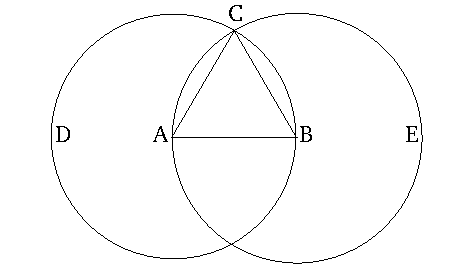
\includegraphics[scale=0.7]{circle}
%\caption{}
%\label{fig:prop 34}
\end{figure}

\noindent Definition of Circle: A Circle is a plane figure contained by one line, such that all of the straight-lines falling upon it from one point among those lying within the figure are equal to one another

\end{document}

